\documentclass[handout]{beamer}
\usepackage{epstopdf}
\usepackage{amsfonts}
\usepackage{amssymb}
\usepackage{amsmath}

\usepackage{subfig}
\newcommand{\vk}{\ensuremath{\mathbf{k}}}
\providecommand{\vr}{\ensuremath{\mathbf{r}}}
%\newcommand{\vec}[1]{\ensuremath{\mathbf{#1}}}

\newcommand{\gk}{\ensuremath{{g}(\mathbf{k})}}

\newcommand{\vp}{\ensuremath{\mathbf{p}}}
\newcommand{\gp}{\ensuremath{{g}(\mathbf{p})}}

\newcommand{\vq}{\ensuremath{\mathbf{q}}}

\newcommand{\Fo}{\ensuremath{\mathbf{F_0}}}


\newcommand{\E}{\ensuremath{\mathbf{E}}}
\newcommand{\A}{\ensuremath{\mathbf{A}}}
\newcommand{\J}{\ensuremath{\mathcal{J}}}

\newcommand{\ket}[1]{\ensuremath{\left|#1\right>}}
\newcommand{\bra}[1]{\ensuremath{\left<#1\right|}}

\newcommand{\twoe}{\ensuremath{2\epsilon_\vk-\E_1}}

\newcommand{\nth}[1]{\ensuremath{\frac{1}{#1}}}

\newcommand{\br}[1]{\ensuremath{\left(#1\right)}}
\newcommand{\mbr}[1]{\ensuremath{\left[#1\right]}}
\newcommand{\bbr}[1]{\ensuremath{\left\{#1\right\}}}


\newcommand{\tk}{\ensuremath{\tilde{k}}}

\newcommand{\kp}{\ensuremath{\ket{\Psi}}}

\newcommand{\av}[1]{\ensuremath{\bigl<{#1}\bigr>}}
\newcommand{\avv}[2][\nu]{\av{#1{\lvert{#2}\rvert}#1}}
\newcommand{\avt}[2]{\av{{#1}|{#2}}}
\newcommand{\avtu}[1]{\av{T_\tau#1}}

\newcommand{\Bop}{\ensuremath{\mathbf{B_0^+}}}
\newcommand{\Bmp}{\ensuremath{\mathbf{B_m^+}}}
\newcommand{\Bnp}{\ensuremath{\mathbf{B_n^+}}}
\newcommand{\Bo}{\ensuremath{\mathbf{B_0}}}
\newcommand{\Bopn}{\ensuremath{\mathbf{{B_0^+}^n}}}
\newcommand{\Bon}{\ensuremath{\mathbf{{B_0}^n}}}


\newcommand{\zmatrix}{\ensuremath{\br{\begin{smallmatrix}0&0\\0&0\end{smallmatrix}}}}
\newcommand{\fmtrx}[4]{\ensuremath{\br{\begin{smallmatrix}#1&#2\\#3&#4\end{smallmatrix}}}}
\newcommand{\smtrx}[6]{\ensuremath{\br{\begin{smallmatrix}#1&#2\\#3&#4\\#5&#6\end{smallmatrix}}}}

\newcommand{\vz}{\ensuremath{v^{\beta\alpha}_{\vk,\vk}}}
%\newcommand{\fz}{

\providecommand{\abs}[1]{\ensuremath{\lvert{#1}\rvert}}

\newcommand{\sg}[1][1]{\ensuremath{\sigma_\frac{#1}{2}}}

\newcommand{\rhof}{\ensuremath{\rho(\ef)}}
\newcommand{\omt}{\ensuremath{\tilde{\Omega}}}
\newcommand{\cht}{\ensuremath{\tilde{\chi_0}}}
\newcommand{\Atl}{\ensuremath{\abs{A}^{2l}}}
\newcommand{\ef}{\ensuremath{\epsilon_F}}

\newcommand{\lca}{\ensuremath{\ln\br{1+\frac{\cht}{\alpha}}}}

\newcommand{\com}[2]{\ensuremath{\mbr{#1,#2}}}
\newcommand{\D}{\ensuremath{\mathit{D}}}
\newcommand{\dg}{\ensuremath{\dagger}}

\providecommand{\lvk}{\ensuremath{1/\vk_F}}
\providecommand{\hm}{\ensuremath{\frac{\hbar^2}}{2m}}
\providecommand{\pdiff}[2]{\ensuremath{\frac{\partial{#1}}{\partial{#2}}}}
\providecommand{\dpdiff}[2]{\ensuremath{\frac{\partial^2{#1}}{\partial{{#2}^2}}}}

\providecommand{\H}{\ensuremath{\mathcal{H}}}
\providecommand{\wt}[1]{\widetilde{#1}}


% \usepackage{beamerthemesplit} // Activate for custom appearance

\title[Crossover w/ 3-species]{BEC-BCS Crossover with the Feshbach Resonance for a Three-Hyperfine-Species Model}
\author[Guojun Zhu]{Guojun Zhu}
\institute{University of Illinois at Urbana-Champaign}
\date{Dec. 15th, 2011}
%\usetheme[language=english,
%titlepagelogo=logopolito, bullet=circle, pageofpages=of, titleline=true, color=blue
%]{TorinoTh}
%\rel{Anthony J. Leggett}
%\usetheme{PaloAlto}
\usetheme{Hannover}
\usecolortheme{whale}
%\AtBeginSection[]
%{
%  \begin{frame}
%    \frametitle{Table of Contents}
%    \tableofcontents[currentsection]
%  \end{frame}
%}
\begin{document}

\frame{\titlepage}

\section[Outline]{}
\frame{\tableofcontents}

\section{Introduction}
%\frame
%{
%  \frametitle{Features of the Beamer Class}
%
%  \begin{itemize}
%  \item<1-> Normal LaTeX class.
%  \item<2-> Easy overlays.
%  \item<3-> No external programs needed.      
%  \end{itemize}
%}

\frame{
\frametitle{Problems}
\begin{itemize}[<+->]
\item General narrow vs broad
\item Three species, interchannel Pauli exclusion
\end{itemize}
}
\section[Atomic Ham.]{Dilute ultracold alkali gas}\label{sec:intro:one}
\frame{
Single Atom Hamiltonian (in spins)
\begin{equation}
\begin{split}\label{eq:intro:1atom}
H_{spin}&=A \mathbf{I}\cdot\mathbf{S}-\mu_{e}\mathbf{B}\cdot\mathbf{S}-{\mu}_{n}\mathbf{B}\cdot\mathbf{I}\\
&=A \mathbf{I}\cdot\mathbf{S}-\mu_{e}{B}{S_{z}}-{\mu}_{n}{B}{I_{z}}
\end{split}
\end{equation}
\begin{itemize}[<+->]
\item Diagonized by total angular momentum at the  zero magnetic field $(F,F_{z})$ 
\begin{equation}
\mathbf{F}=\mathbf{S}+\mathbf{I}
\end{equation}

\item $(F,F_{z})$  are no longer eigenstate at a finite magnetic field. 

\end{itemize}
}
\frame{
\begin{figure}[htbp]
\begin{center}
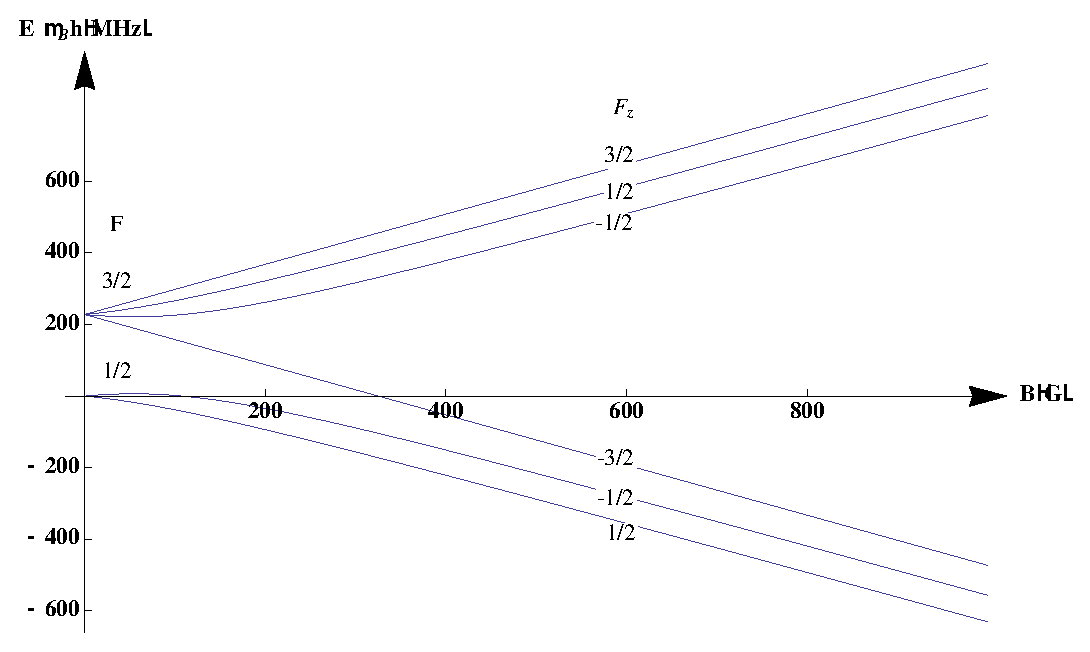
\includegraphics[width=0.8\textwidth]{hyperfineLi6}
\caption{Hyperfine structure of a single \textsuperscript{6}Li atom } 
Levels are marked with $F$ and $F_{z}$ {(see Footnote \ref{foot:intro:f} in page \pageref{foot:intro:f})} %Note that the energy of the $\ket{F=\nth{2},F_z=-\nth{2}}$ state first increases with the magnetic field, $B$, at low field then decrease at high field. In the same way, the energy of the $\ket{F=\frac{3}{2},F_z=-\nth{2}}$ state first decreases and then increases with the magnetic field.  
\label{fig:intro:li6}
\end{center}
\end{figure}
}

\frame{
\frametitle{Interaction between two atoms}

\begin{itemize}[<+->]
\item Channels: one  configuration of hyperfine spins for one atom pair in interaction, $\ket{F^{(1)},F_{z}^{(1)}}\otimes\ket{F^{(2)},F_{z}^{(2)}}$ 
\item Interaction mostly due to electrons
\begin{equation}\label{eq:intro:two}
V=f(r)+g(r)\mathbf{S_{1}}\cdot\mathbf{S_{2}}
\end{equation}
\item Channels are mixed. 
\item In high field, channels are good zeroth approximation
\end{itemize}

}
 \section[2-body]{The  Feshbach resonance in two-body physics\label{sec:intro:twobody}}
\frame{
\begin{figure}[htbp]
\begin{center}
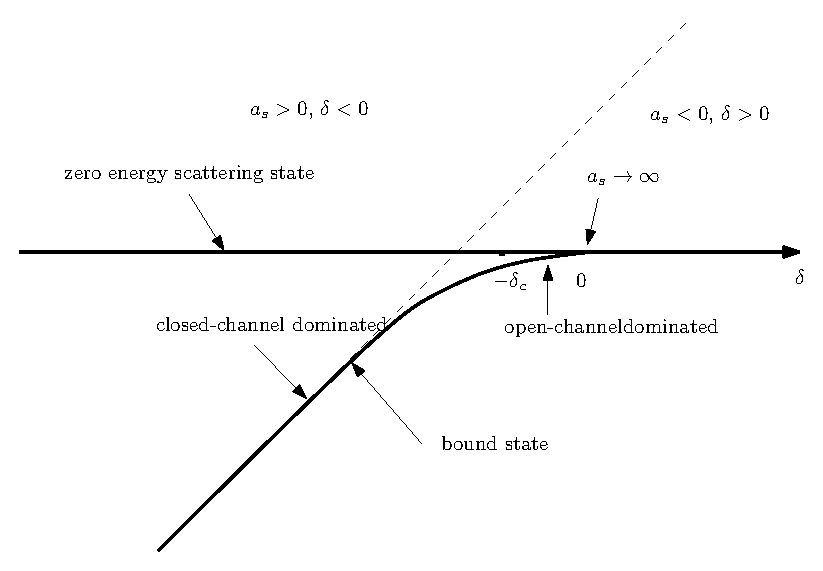
\includegraphics[width=0.8\textwidth]{levels}
\caption{Energy levels in a Feshbach resonance\label{fig:intro:levels}} 
\parbox{0.9\textwidth}{\small $\delta$ is the energy detuning from the resonance point, where the resonant point is defined as the point where the open-channel effective s-wave scattering length diverges, $a_s\to\pm\infty$.  The horizontal line stands for the zero energy s-wave scattering state, $\psi\sim\nth{r}-\nth{a_s}$, which exists for any detuning.  The lower line stands for the real bound state, which only exists for negative detuning ($\delta<0$, $a_s>0$). The dash line stands for the (uncoupled) closed-channel bound state.  An interesting point to notice is that the real bound state appears earlier than the cross point of the (uncoupled) closed-channel bound state level and zero energy. Another important point to notice is the negative detuning $-\delta_c$.  When the negative detuning is smaller than $\delta_c$, this real bound state is composed mostly with atoms in the open-channel and vice verse.  See Chapter \ref{sec:intro:twobody} for details about $\mathcal{K}$ and $\delta_c$.   }

\end{center}
\end{figure}
}
\begin{frame}
        \frametitle{`Hidden higher-order concepts?'}
        \begin{itemize}[<+->]
        \item The truths of arithmetic which are independent of PA in some 
        sense themselves `{contain} essentially {\color{blue}{hidden higher-order}},
         or infinitary, concepts'???
        \item `Truths in the language of arithmetic which \ldots
        \item That suggests stronger version of Isaacson's thesis. 
        \end{itemize}
\end{frame}
\frame{
	\frametitle{No interchannel exclusion}
	\begin{gather}
1=-\mbr{\frac{4\pi{\tilde{a}_{s}(\mu)}}{m}\sum(\nth{2E_{\vk}}-\nth{2\epsilon_{\vk}})}\label{eq:pathInt2:narrowGapS}\\
N_{\text{open}}=\sum_\vk\frac{E_\vk-\xi_\vk}{2E_\vk}\label{eq:pathInt2:narrowNumS}
\end{gather}
}
\frame{
\begin{figure}[htbp]
\begin{center}
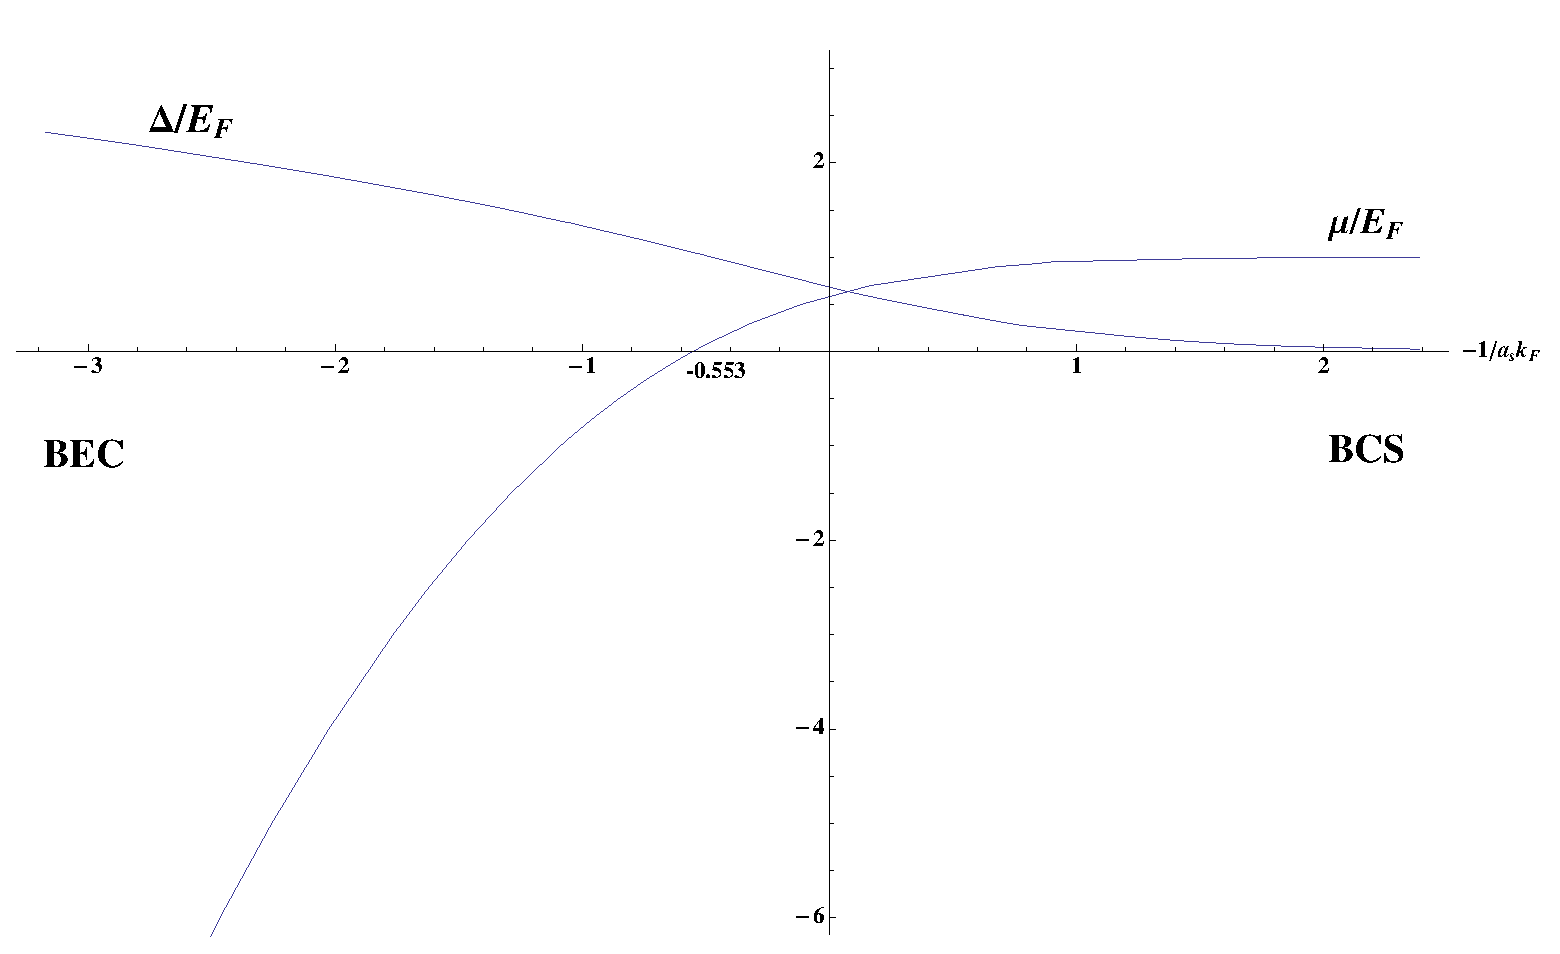
\includegraphics[width=0.8\textwidth]{SingleChannelCrossoverMuDelta}
\caption{The chemical potential $\mu$ and gap $\Delta$ in the mean field level over crossover} 
\label{fig:pathInt:meanField}
{\small All quantities in the unit of energy ($\mu$, $\Delta$) are rescaled with the Fermi energy $E_{F}$ and the s-wave scattering length $a_{s}$ is rescaled with $1/k_{F}$.  }
\end{center}
\end{figure}
}
\section{Mean-field result}
\frame{
\begin{figure}[hhtb]
	\centering
	         \subfloat[$E_{F}<\tilde\delta$]{\label{fig:narrowFR:aboveSea}\includegraphics[width=.2\textwidth]{narrowFRabove.eps}}\quad
		\subfloat[$0<\tilde\delta<E_{F}$]{\includegraphics[width=.30\textwidth]{narrowFRin.eps}\label{fig:narrowFR:inSea}}\quad
		\subfloat[$\tilde\delta<0$]{\label{fig:narrowFR:belowSea}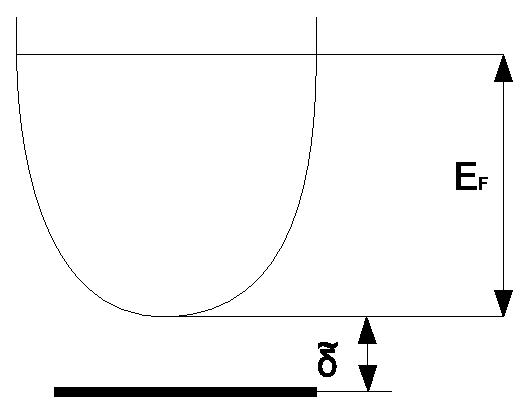
\includegraphics[width=.20\textwidth]{narrowFRbelow.eps}}
	\caption{Extremely narrow resonance\label{fig:narrowFR}}
	\small{The shaded area is occupied by atoms. }
	%\parbox{0.7\textwidth}{\small{  In Fig. \subref{fig:narrowFR:inSea} chemical potential would be close to the closed-channel bound state level (besides small shift due to the open-channel intra-channel coupling) and the ``Fermi sea'' above is empty. }}
\end{figure}}
\frame{
\begin{figure}[htbp]
\begin{center}
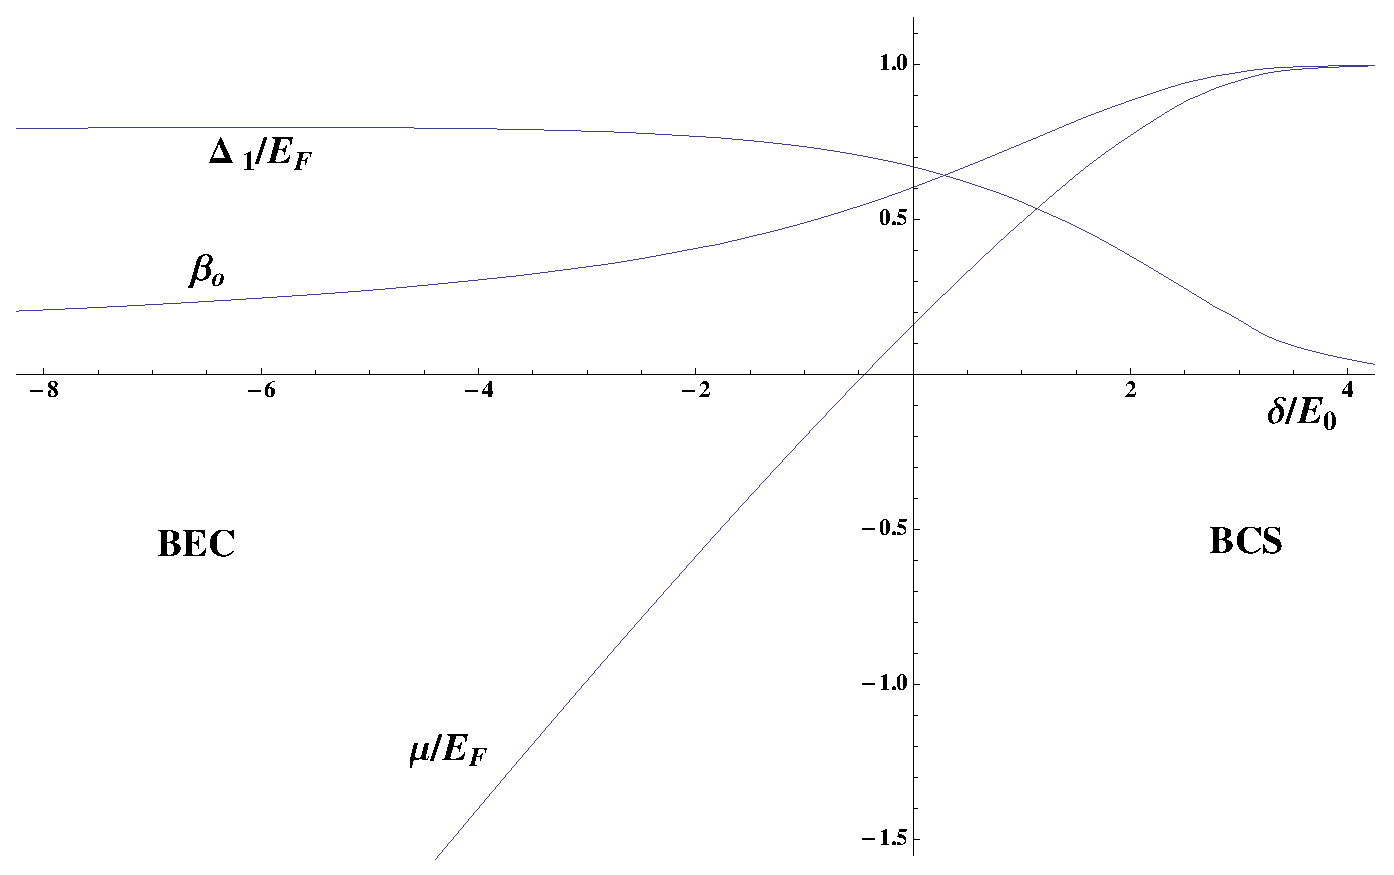
\includegraphics[width=0.8\textwidth]{narrow}
\caption{The chemical potential $\mu$, the open-channel gap $\Delta_{1}$ and the open-channel relative weight $\beta_{o}$ over crossover with the narrow Feshbach resonance without considering the inter-channel Pauli exclusion  vs. the chemical potential and the gap in the single-channel model} 
\label{fig:pathInt2:narrow}
{\small  The gap in the open-channel $\Delta_{1}$ and the chemical potential $\mu$ are rescaled with the the Fermi energy of the total density, $E_{F}^{(tot)}$.  The $x$-axis is the detuning $\delta$ rescaled with $E_{0}$ (see Eq. \ref{eq:pathInt2:E0}) for the narrow resonance; while it is $-1/a_{s}k_{F}$ for the single-channel curves. We have taken $\delta_{c}=0.001E_{F}^{(tot)}$ for the narrow resonance figure. We used the detuning from the resonant point  for the $x$-axis in the narrow resonance instead of $-1/a_{s}k_{F}$ in the single-channel because the additional shift, $2\mu$, considering in Eq. \ref{eq:pathInt2:simplenarrowAs}.  Consequently, the chemical potential lines in both cases cross the $x$-axis at the same point where $\mu=0$.  }
\end{center}
\end{figure}
}
\section{Excitation Mode}
\frame{}
\section{Conclusion}
\frame{}
\bibliography{../citation}
\bibliographystyle{apalike}
\end{document}
